% *======================================================================*
%  Cactus Thorn template for ThornGuide documentation
%  Author: Ian Kelley
%  Date: Sun Jun 02, 2002
%  $Header$
%
%  Thorn documentation in the latex file doc/documentation.tex 
%  will be included in ThornGuides built with the Cactus make system.
%  The scripts employed by the make system automatically include 
%  pages about variables, parameters and scheduling parsed from the 
%  relevent thorn CCL files.
%  
%  This template contains guidelines which help to assure that your     
%  documentation will be correctly added to ThornGuides. More 
%  information is available in the Cactus UsersGuide.
%                                                    
%  Guidelines:
%   - Do not change anything before the line
%       % BEGIN CACTUS THORNGUIDE",
%     except for filling in the title, author, date etc. fields.
%        - Each of these fields should only be on ONE line.
%        - Author names should be sparated with a \\ or a comma
%   - You can define your own macros are OK, but they must appear after
%     the BEGIN CACTUS THORNGUIDE line, and do not redefine standard 
%     latex commands.
%   - To avoid name clashes with other thorns, 'labels', 'citations', 
%     'references', and 'image' names should conform to the following 
%     convention:          
%       ARRANGEMENT_THORN_LABEL
%     For example, an image wave.eps in the arrangement CactusWave and 
%     thorn WaveToyC should be renamed to CactusWave_WaveToyC_wave.eps
%   - Graphics should only be included using the graphix package. 
%     More specifically, with the "includegraphics" command. Do
%     not specify any graphic file extensions in your .tex file. This 
%     will allow us (later) to create a PDF version of the ThornGuide
%     via pdflatex. |
%   - References should be included with the latex "bibitem" command. 
%   - use \begin{abstract}...\end{abstract} instead of \abstract{...}
%   - For the benefit of our Perl scripts, and for future extensions, 
%     please use simple latex.     
%
% *======================================================================* 
% 
% Example of including a graphic image:
%    \begin{figure}[ht]
% 	\begin{center}
%    	   \includegraphics[width=6cm]{MyArrangement_MyThorn_MyFigure}
% 	\end{center}
% 	\caption{Illustration of this and that}
% 	\label{MyArrangement_MyThorn_MyLabel}
%    \end{figure}
%
% Example of using a label:
%   \label{MyArrangement_MyThorn_MyLabel}
%
% Example of a citation:
%    \cite{MyArrangement_MyThorn_Author99}
%
% Example of including a reference
%   \bibitem{MyArrangement_MyThorn_Author99}
%   {J. Author, {\em The Title of the Book, Journal, or periodical}, 1 (1999), 
%   1--16. {\tt http://www.nowhere.com/}}
%
% *======================================================================* 

% If you are using CVS use this line to give version information
% $Header$

\documentclass{article}

% Use the Cactus ThornGuide style file
% (Automatically used from Cactus distribution, if you have a 
%  thorn without the Cactus Flesh download this from the Cactus
%  homepage at www.cactuscode.org)
\usepackage{../../../../doc/latex/cactus}

%%%%%%%%%%%%%%%%%%%%%%%%%%%%%%%%%%%%%%%%%%%%%%%%%%%%%%%%%%%%%%%%%%%%%%%%%%%%%%%%

\begin{document}

\author{Original code and documentation by Peter Diener}

% The title of the document (not necessarily the name of the Thorn)
\title{Thorn Guide for the {\tt EHFinder} Thorn}

% the date your document was last changed, if your document is in CVS, 
% please use:
%    \date{$ $Date$ $}
\date{$ $Date$ $}

\maketitle

% Do not delete next line
% START CACTUS THORNGUIDE

% Add all definitions used in this documentation here 
%   \def\mydef etc

% force a line break in a itemize/description/enumerate environment
\def\forcelinebreak{\mbox{}\\[-\baselineskip]}

\def\defn#1{{\bf #1}}

\def\eg{e.g.\hbox{}}
\def\ie{i.e.\hbox{}}
\def\etal{{\it et~al.\/\hbox{}}}
\def\nb{n.b.\hbox{}}
\def\Nb{N.b.\hbox{}}

% math stuff
\def\diag{\text{diag}}
\def\Gaussian{{\sf G}}
\def\half{{\textstyle \frac{1}{2}}}
\def\sech{\text{sech}}

% Add an abstract for this thorn's documentation
\begin{abstract}
This thorn locates the Event Horizon (EH) in an analytic or numerical spacetime
by evolving a null surface backwards in time. The null surface is described at
each time step as the 0-level iso-surface of a 3D scalar function $f$. This
level set description of the surface allows, trivially, changes of the topology
of the surface so it is possible to follow the merger of two (or more) black
holes into a final black hole.

\end{abstract}

%%%%%%%%%%%%%%%%%%%%%%%%%%%%%%%%%%%%%%%%%%%%%%%%%%%%%%%%%%%%%%%%%%%%%%%%%%%%%%%%

\section{Introduction}
This thorn attempts to locate the Event Horizon (EH) in an analytic or
numerical spacetime by evolving a null surface backwards in time. This
method depends on the fact that, except in cases where the coordinates are
adapted to outgoing null geodesics, an outgoing null surface started close
to the EH, when evolved forward in time, is diverging exponentially from the
EH. Reversing the time evolution then means that an outgoing null surface
will converge exponentially to the EH. The level set function, $f$, is
evolved according to
\begin{eqnarray}
\partial_{t}f & = & \frac{-g^{ti}\partial_{i}f+\sqrt{(g^{ti}\partial_{i}f)^{2}-
g^{tt}g^{ij}\partial_{i}f\partial_{j}f}}{g^{tt}} \nonumber \\
 & = & \beta^{i}\partial_{i}f-
                \sqrt{\alpha^{2}\gamma^{ij}\partial_{i}f\partial_{j}f},
\label{AEIThorns_EHFinder_evolve}
\end{eqnarray}
where in the second equation the lapse, shift and 3-metric has been substituted
for the 4-metric. For more details on the theory and implementation
see~\cite{AEIThorns_EHFinder_Diener02}.

This thorn uses a level set description of the null surface, \ie the surface
is the 0-level isosurface of a 3D scalar function, $f$, that is negative
inside and positive outside the surface. With this choice of surface
description one level-set function can describe multiple surfaces at the
same time, simply by having several, disconnected regions with negative
values. The biggest advantage, however, is that any change of topology of
the surface is handled naturally and simply by the level-set function
changing sign. Therefore this {\tt EHFinder} can follow the EH during the
merger of two (or more) black holes into one black hole.

To find the EH in a numerical spacetime several points have to be taken into
consideration. Since the null surface has to be evolved backwards in time, the
{\tt EHFinder} has to be seen as a pre-processing analysis thorn. Therefore it
is necessary to evolve the initial data forward in time while outputting
enough 3D data, that the full 4-metric can be recovered at each timestep.
The 3D data is then read back in, in reverse order, while the level-set
function is evolved backwards in time. The thorn can evolve more than one
level set function at a time using different initial guesses for the surfaces
(NOTE: this is a quite recent feature and has not yet been tested extensively).
More details about the actual use of the thorn in
 section~\ref{AEIThorns_EHFinder_UseThorn}

\section{Re-initialization}
\label{AEIThorns_EHFinder_re_init}
The evolution equation for $f$, 
equation~(\ref{AEIThorns_EHFinder_evolve}), causes steepening of
the gradient of $f$, which is undesireble numerically. For that reason, $f$
is periodically re-initialized to a distance function. That is, the values of
$f$ are changed so that the the value of $f$ in a grid point is equal to the
(signed) distance from the grid point to the surface $f=0$. This is done by
evolving $f$ according to the following evolution equation (in the parameter
$\lambda$)
\begin{equation}
\frac{df}{d\lambda} = -\frac{f}{\sqrt{f^{2}+1}}\left (|\nabla f|-1\right )
\label{AEIThorns_EHFinder_reinit}
\end{equation}
until a steady state is achieved. This method is called the {\tt pde}-method
since it is basically evolving a pde. Sometimes the $f=0$ surface can be
moved slightly during the re-initialization procedure. This happens when
the surface develops a narrow neck just before a topology change. For
that reason, there is an option to detect when this is about to happen and
undo the re-initialization.

There used to be another method doing the re-initialization, but it proved
inferior to the {\tt pde}-method and was removed. Other methods may be
implemented in the future.

\section{The initial shape of the surface}
\label{AEIThorns_EHFinder_initial}
Currently three different choices for the initial shape of the surface are
implemented. The simplest choice is a sphere in which case $f$ is set
according to
\begin{equation}
f = \sqrt{(x-x_{0})^2+(y-y_{0})^2+(z-z_{0})^2} - r_{0},
\label{AEIThorns_EHFinder_sphere}
\end{equation}
where $r_{0}$ is the radius of the sphere and $x_{0}$, $y_{0}$ and $z_{0}$
are the coordinates of the center of the sphere. The second choice is a rotated
and translated ellipsoid. The basic equation is here
\begin{equation}
f = \sqrt{\frac{x^{2}}{a^{2}}+\frac{y^{2}}{b^{2}}+\frac{z^{2}}{c^{2}}} - 1
\label{AEIThorns_EHFinder_ellipsoid}
\end{equation}
This ellipsoid is first rotated an angle $\alpha$ around the $z$-axis, then
rotated an angle $\beta$ around the $y$-axis, then rotated an angle $\gamma$
around the $x$-axis and finally the rotated ellipsoid is translated to have
its ``center'' at the point $(x_{0},y_{0},z_{0})$. The final possible shape
of the initial surface is an ovaloid of Cassini. This was implented initially
to test changing the topology in flat space. it is most likely not useful for
numerical data. In this case $f$ is set according to
\begin{equation}
f = (x^{2}+y^{2}+z^{2})^{2} + a^{4} - 2 a^{2} (x^{2}-y^{2}-z^{2})-b^{4}.
\label{AEIThorns_EHFinder_cassini}
\end{equation}
There are no translation or rotations implemented for the ovaloid of Cassini.

Different initial shapes can be used for the different level set functions
used in the same run.
\section{Excision}
\label{AEIThorns_EHFinder_excise}

Even though the level set function, $f$, in principle can be defined
everywhere it is often advantageous to only evolve it in a certain region
around the surface $f=0$. Since $f$ is re-initialized regularly to become
a distance function, $f$ itself can be used as a measure of the distance
from a certain grid point to the surface $f=0$. The parameter
{\tt ehfinder::shell\_width} specifies the size of the active region
around $f=0$. However the interior and exterior excisions are handled
differently. The interior excision is most simple, since here all grid points
with $f<-{\mbox{\tt ehfinder::shell\_width}}$ are marked as inactive. This
should work in all cases when the excised region is everywhere concave, since
then all points on the boundary of the excised region will have enough
neighbouring active points to be able to calculate second order accurate one
sided derivatives. If the interior excised region happens to have a convex
region, this might fail. To avoid a similiar problem at the outer excised
boundary, this boundary is shaped as a rectangular box. The box is chosen
so that all points with $f<{\mbox{\tt ehfinder::shell\_width}}$ are in the
active region. This is illustrated in
Figure~\ref{AEIThorns_EHFinder_excisefig}, for the case
\begin{figure}[ht]
  \begin{center}
    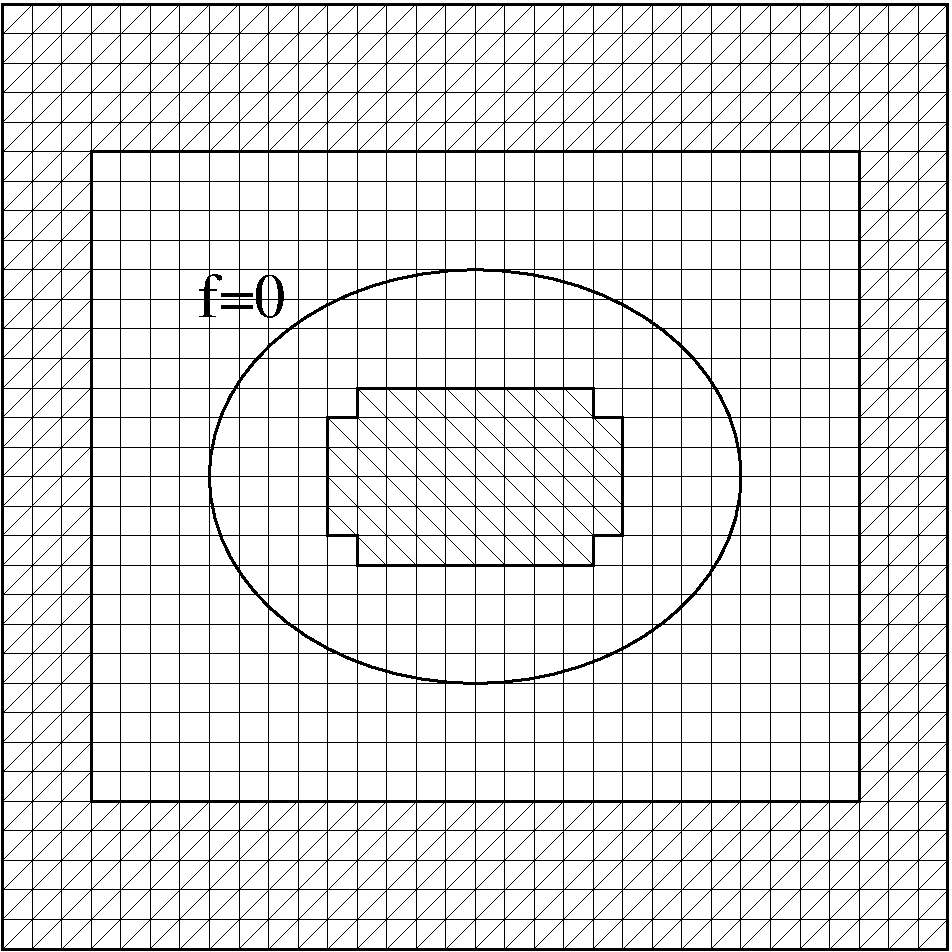
\includegraphics[width=8cm]{excision}
  \end{center}
  \caption{Illustration of the excision regions used internally by
           {\tt EHFinder}. The hashed regions are excised.}
  \label{AEIThorns_EHFinder_excisefig}
\end{figure}
{\tt ehfinder::shell\_width = 4}, where the excised regions are hashed.

Changes to the excision regions are only done after re-initialization,
since it is only at this time that $f$ is a distance function. The excision
regions can move across the grid, tracking the surface $f=0$.

Also if the numerical run was done with excision using {\tt SpaceMask},
the {\tt EHFinder} excision region is guaranteed to completely cover the 
numerical excision region. The {\tt EHFinder} currently only supports the
old style excision mask but the support of the new style excision mask
should be trivial and fast to implement.
\section{Upwinding}
\label{AEIThorns_EHFinder_upwind}
All finite differences used in the evolution of the null surface are second
order one sided differences. For that reason a {\tt ghost\_size} larger or
equal to 2 should always be used. It is possible to choose between three
different upwinding schemes. This is done by setting the parameter
{\tt ehfinder::upwind\_type} to either {\tt intrinsic}, {\tt shift} or
{\tt characteristic}.

The {\tt intrinsic} scheme, looks at the values of $f$ itself, to determine
the direction of the stencil. This is basically in order to be able to handle
situations like the one illustrated in 1D in
Figure~\ref{AEIThorns_EHFinder_upwindfig}.
\begin{figure}[ht]
  \begin{center}
    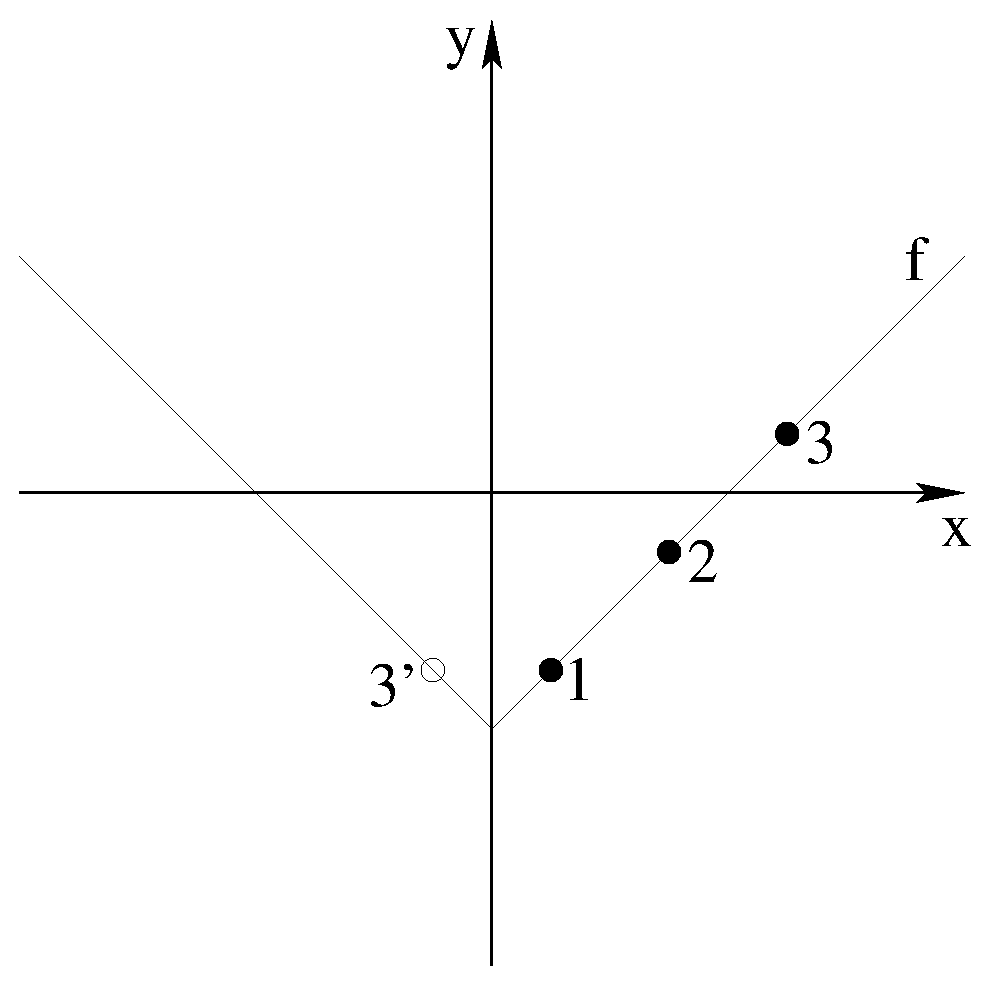
\includegraphics[width=8cm]{upwind}
  \end{center}
  \caption{An illustration of how to choose the upwinding stencil when $f$
           is not differntiable everywhere}
  \label{AEIThorns_EHFinder_upwindfig}
\end{figure}
If the stencil for calculating derivatives in the point labeled 1 is taken
to consist of the points 1, 2 and 3', the non differentiablility of $f$ may
cause problems. The algorithm detects this and instead uses the points 1, 2, 3
as the stencil. This ensures that a non differentiable feature can be
maintained in the evolution.

However this scheme only works in a few simple cases. For more general cases
it is important to use characteristic information in order to ensure that
the numerical stencil contains the domain of dependence. Therefore the
{\tt characteristic} scheme was introduced. Fortunately, by using the
information contained in the level set functions the characteristic of
the level set function can be calculated using
\begin{equation}
\frac{dx^{i}}{dt}=-\beta^{i}+\frac{\alpha^{2}\gamma^{ij}\partial_{j}f}
{\sqrt{\alpha^{2}\gamma^{kl}\partial_{k}f\partial_{l}f}}. 
\label{eq:char}
\end{equation}
The method estimates the characteristic direction using centered finite
differences in equation~(\ref{eq:char}) and then recalculates the one
sided finite differences in the appropriate direction.

It might happen that the upwinding direction based on the characteristic
direction results in the stencil to consist of the points 1, 2, 3' in 
Figure~\ref{AEIThorns_EHFinder_upwindfig}. However, if the 
re-initialization is done often enough, this turns out not to cause
any problems.

The {\tt shift} scheme was implemented as an improvement to the {\tt intrinsic}
scheme but it turned out that the {\tt characteristic} scheme was superior.
Therefore {\tt shift} upwinding should not be used. It might be completely
removed in future revisions.

For the re-initialization the default is to use the {\tt intrinsic} 
second order scheme (the re-initialization doesn't depend on where the
surface is moving), so {\tt characteristic} upwinding is not applicable.
It is possible to use a first order {\tt intrinsic} scheme, but this is, in my
experience, not accurate enough. A centered differencing scheme is also
available, but is only there for testing purposes and should never be used.
These alternative schemes will probably be removed in the future.

\section{The most important parameters}
Here the most important parameters are described.
\begin{itemize}
\item {\tt ehfinder::mode} \\  
  The mode can either be set to {\tt normal} (normal event horizon finder
  mode), {\tt analysis} (compare a previously calculated level set function to
  a small number of analytic spacetimes) and {\tt generator} (only evolve
  the generators while keeping the level set function fixed). The
  default is {\tt normal} and should normally not be changed. The other modes
  are only useful for debugging and testing purposes.
\item{\tt ehfinder::eh\_number\_level\_sets} \\
  An integer parameter specifying how many individual level set functions to
  evolve at a time. Currently it has to be between 1 and 10.
\item {\tt ehfinder::eh\_metric\_type} \\
  The metric type can either be set to {\tt numerical} or {\tt analytic}. If
  it is set to {\tt numerical} the {\tt EHFinder} will attempt to read in the
  metric from files in the directory specified by the {\tt io::recover\_dir}
  parameter. At present all the timesteps has to be saved in the same file.
  Note that if the numerical data was produced with
  {\tt admbase::metric\_type = "static conformal"} this parameter has to be
  specified again. In this case the {\tt EHFinder} will attempt to also read
  in the conformal factor from a file.
  If metric type is set to {\tt analytic} another thorn needs to set up the
  metric. It is possible to only set the metric on the initial slice, but it
  is also possible to have a thorn (like thorn {\tt Exact}) set the metric at
  {\tt CCTK\_PRESTEP} if the analytic metric is time dependent.
  The default is {\tt numerical}.
\item {\tt ehfinder::eh\_lapse\_type} \\
  The same for the lapse.
\item {\tt ehfinder::eh\_shift\_type} \\
  The same for the shift.
\item {\tt initial\_f[i]} \\
  A vector parameter specifying the initial shape of the null surface for
  the individual level set functions. The initial shape can currently be
  chosen from {\tt sphere}, {\tt ellipsoid} and {\tt cassini} as described in
  section~\ref{AEIThorns_EHFinder_initial}. The default is {\tt sphere}.
\item {\tt initial\_rad[i]} \\
  A vector parameter specifying the radius of the initial sphere ($r_{0}$ in
  equation~\ref{AEIThorns_EHFinder_sphere}). The deafault is 1.
\item {\tt translate\_x[i]} \\
  A vector parameter specifying how much to translate the initial surface in
  the $x$-direction ($x_{0}$ in equation~\ref{AEIThorns_EHFinder_sphere}).
  Also used for the initial ellipsoid. The default is 0.
\item {\tt translate\_y[i]} \\
  A vector parameter specifying how much to translate the initial surface in
  the $y$-direction ($y_{0}$ in equation~\ref{AEIThorns_EHFinder_sphere}).
  Also used for the initial ellipsoid. The default is 0.
\item {\tt translate\_z[i]} \\
  A vector parameter specifying how much to translate the initial surface in
  the $z$-direction ($z_{0}$ in equation~\ref{AEIThorns_EHFinder_sphere}).
  Also used for the initial ellipsoid. The default is 0.
\item {\tt initial\_a[i]} \\
  A vector parameter specifying $a$ in
  equation~\ref{AEIThorns_EHFinder_ellipsoid}. The default is 1.
\item {\tt initial\_b[i]} \\
  A vector parameter specifying $b$ in
  equation~\ref{AEIThorns_EHFinder_ellipsoid}. The default is 1.
\item {\tt initial\_c[i]} \\
  A vector parameter specifying $c$ in
  equation~\ref{AEIThorns_EHFinder_ellipsoid}. The default is 1.
\item {\tt rotation\_alpha[i]} \\
  A vector parameter specifying the rotation angle $\alpha$ for the ellipsoid
  around the $z$-axis. The default is 0.
\item {\tt rotation\_beta[i]} \\
  A vector parameter specifying the rotation angle $\beta$ for the ellipsoid
  around the $y$-axis. The default is 0.
\item {\tt rotation\_gamma[i]} \\
  A vector parameter specifying the rotation angle $\gamma$ for the ellipsoid
  around the $x$-axis. The default is 0.
\item {\tt shell\_width} \\
  The width of the active evolution region. Grid points more than
  {\tt shell\_width} gridspacings away from the $f=0$ surface are marked
  as inactive and are not evolved as described in
  section~\ref{AEIThorns_EHFinder_excise}. The default is $7$
  gridspacings.
\item {\tt use\_inner\_excision} \\
  A boolean parameter specifying whether the interior excision should be
  used or not.
\item {\tt use\_outer\_excision} \\
  A boolean parameter specifying whether the exterior excision should be
  used or not.
\item {\tt upwind\_type} \\
  The type of upwinding to be used (either {\tt intrinsic}, {\tt shift} or 
  {\tt characteristic}). See the detailed description of the upwinding types
  in section~\ref{AEIThorns_EHFinder_upwind}. The default is 
  {\tt characteristic}.
\item {\tt surface\_direction} \\
  The code can track both outgoing and ingoing null surfaces. Choose the 
  direction by using {\tt outward} or {\tt inward}. The default is
  {\tt outward}. Note that the code only works as an event horizon finder
  when evolving outward going null surfaces backwards in time.
\item {\tt re\_init\_undo} \\
  Should the re-initialization be undone just before pinch-off or not as
  described in section~\ref{AEIThorns_EHFinder_re_init}. The
  default is {\tt "no"}.
\item {\tt re\_init\_int\_method} \\
  Choose the integration method in the {\tt pde}-re-initialization method.
  Choose either a simple Euler ({\tt euler}) integration scheme or a second
  order Runge-Kutta ({\tt rk2}) scheme. Since a pde is evolved to steady state,
  it seems that the Euler scheme works just fine and is faster than the
  Runge-Kutta scheme. The default is {\tt euler}.
\item {\tt re\_init\_max\_iter} \\
  The maximum number of iterations in the {\tt pde}-re-initialization scheme,
  before giving up. Unless you are working at high resolution the default
  should be enough. The default is 800.
\item {\tt pde\_differences} \\
  Choose the type of finite differencing used in the {\tt pde}
  re-initialization. Don't ever use anything else than second order
  upwinding ({\tt upwind2}). The other choices ({\tt centered} and {\tt upwind})
  are there only for testing purposes and might be removed.
\item {\tt re\_initialize\_every} \\
  How often to re-initialize using the {\tt pde} re-initialization. This
  depends on the problem. For some problems it is necessary to do it more
  often than for other problems. You'll have to experiment to figure out
  what works best. The default is 10.
\item {\tt last\_iteration\_number} \\
  The last iteration number of the numerical
  simulation that produced the metric data. Active when {\tt eh\_metric\_type}
  is equal to {\tt numerical}.
\item {\tt saved\_iteration\_every} \\
  How often was the numerical data saved?
  This and the above parameter is used in the code to figure out which
  data set iteration number to read in from file \\
  ({\tt last\_iteration\_number-saved\_iteration\_every*cctk\_iteration}).
\item {\tt ntheta} \\
  How many points in the $\theta$-direction should be used for integrations
  over the surface.
\item {\tt nphi} \\
  How many points in the $\phi$-direction should be used for integrations
  over the surface.
\item {\tt maximum\_surface\_number} \\
  The maximal number of surfaces expected at any given time during the whole
  evolution.
\item {\tt surface\_interpolator} \\
  Which interpolator to use for the location of points on the surface. It
  should be the name of a valid interpolator provided by one of the available
  interpolators. The interpolator should be able to return both the
  interpolated value and derivatives. At present this is provided by
  {\tt AEILocalInterp}. The default is {\tt Hermite polynomial interpolation}.
\item {\tt surface\_interpolation\_order} \\
  The interpolation order used for finding points on the surface. Higher
  orders require larger number of ghost zones for parallel runs. The default
  value is 2 (consistent with a ghostsize of 2).
\item {\tt area\_interpolator} \\
  Which interpolator should be used to interpolate metric information onto the
  surface once the surface points have been found. The default is
  {\tt Lagrange polynomial interpolation}.
\item {\tt area\_interpolation\_order} \\
  The interpolation order used for calculating the area of the surface.
  The default value is 3 (consistent with a ghostsize of 2).
\end{itemize}
{\tt EHFinder} also extends the following parameter from {\tt admbase} in order
to be able to read in initial data.
\begin{itemize}
\item {\tt admbase::initial\_data} is extended with {\tt "read from file"}.
\item {\tt admbase::initial\_lapse} is extended with {\tt "read from file"}.
\item {\tt admbase::initial\_shift} is extended with {\tt "read from file"}.
\end{itemize}
\section{How to use {\tt EHFinder} with numerical data}
\label{AEIThorns_EHFinder_UseThorn}
In this section I will try to describe in little more detail how {\tt EHFinder}
can be used to find the EH in a numerical spacetime.

\subsection{Outputting numerical data}
The first thing to make sure, is that enough data is output during the
numerical run, to be able to reconstruct the full 4-metric. The
required output therefore consists of the {\tt ADMBase::metric},
{\tt ADMBase::lapse} and {\tt ADMBase::shift}. However if the evolution was
done with zero shift and/or lapse equal to one, it is not necessary to output
these grid functions, as long as storage is turned on and they are set to the
correct value initially when {\tt EHFinder} is run. If the evolution was done
with a conformal factor then {\tt StaticConformal::psi} has to be output as
well, since it is necessary in order to reconstruct the 4-metric. However it
is only necessary to output this once since it is constant during the evolution.
It is not necessary to output the derivatives of the conformal factor. If
excision was used in the numerical run then it is also necessary to output 
{\tt SpaceMask::emask}\footnote{When more thorns have been converted to use
{\tt SpaceMask::space\_mask} this option will also be supported.}, since
{\tt EHFinder} has to make sure that its internal mask covers the space mask.

At present it is necessary to output all timesteps into the same file (use
{\tt IO::out\_timesteps\_per\_file = -1}, which is the default). In principle
both {\tt FLEXIO} and {\tt HDF5} output should be supported, but only
HDF5 output has been tested. Since {\tt EHFinder} can be run on a lot less
processors compared to the spacetime evolution, it is often advantageous to
either do unchuncked output or to recombine the output files, since it is then
possible to read the data onto a smaller number of processors (use
{\tt IO::out\_unchunked = "yes"} to write unchunked data). If the numerical
run is larger than the EH containing region (hopefully that is the case;
otherwise the boundaries are definitely to close in), it is possible to
use hyperslabbing to just output the EH containing region (see for example
{\tt CactusPUGHIO/IOHDF5} for details on this). If hyperslabbing is used it
is definitely necessary to do the output unchunked or recombine afterwards.
An example parameter file can be seen in the {\tt par/Misner\_2.2\_80\_3D.par}.

In principle {\tt EHFinder} should also work for downsampled (in both space
and time) data, but no experiments have been done so far to estimate the loss
of accuracy (I have always used the full resolution and done output at
every timestep).

If hyperslabbing and/or downsampling is used, it is the users responsibility
(by specifying the right parameters in the parameter file) to ensure that
{\tt EHFinder} is run with the correct grid spacing and time step.

\subsection{Tips for parameter choices}

{\tt EHFinder} is still under development and testing and can as yet {\em not}
be used as a black box. But still I can give some guidelines and advice on
how to proceed.

The first concern is to setup the initial guess for the surface. Ideally one
would like to use at least two different initial surfaces. One surface 
completely inside the EH and one surface completely outside the EH. In
practice it is often a good idea to use more than two different initial
surfaces, since then the initial surfaces closest to the EH can be identified.
Using the feature of evolving multiple level set functions at a time, this
can be done while reading in the numerical data only once. The easiest way
to get an initial surface inside the EH, is to set up the initial guess to
be completely inside the
apparent horizon (AH). To get an initial guess that is outside of the EH
is not as easy. One way is to choose a surface, that starts to contract
everywhere when evolved according to
equation~(\ref{AEIThorns_EHFinder_evolve}). However this is not a
guarantee, since the EH can be expanding in the numerical coordinates.
This of course means that it is necessary to do it by trial and error.
Set up some initial guess evolve it for a little while, look at 3D output
to determine if the surface is contracting everywhere and change the
initial surface if necessary.

Then comes the question of how often to do the re-initialization and how
much to excise. These parameters depend on the numerical data. In principle,
since the re-initialization can move the surface, one wants to do it as
rarely as possible. On the other hand, re-initialization is necessary
in order to keep the evolution nicely controlled (by avoiding large gradients),
so a compromise has to be found. This might require some experimentation.
Because movements of the surface during re-initialization, usually only
occurs close to moments of topology change, it might be necessary to evolve
all the way beyond the change of topology and look at 3D output to see if
any problems occured. If significant movement of the surface during
re-initialization near the change of topology is observed, then try again
with re-initialization undo activated. How often to do the re-initialization
also depends on the width of the active region. If the active region around
the surface is narrow, it might be necessary to re-initialize more often,
since in this case the boundaries of the active region is closer to the
surface. At the boundaries the stencil direction is dictated by the geometry
and not $f$ itself or the characteristics, which might cause instabilities
if it is not re-initialized. Good values guesses for
{\tt ehfinder::reinitialize\_every\_pde} seems to in the range 5--10 at
low or medium resolutions but can usually be increased for higher
resolutions. For {\tt ehfinder::shell\_width} I normally use at least 7.

{\tt EHFinder} does not yet work fully with the fixed mesh refinement driver
{\tt Carpet}, but this is under development. Currently the evolution of the
level set function and the re-initialization works, but only with no inner
and outer excision. The analysis routines to find areas of the surfaces does
not work with {\tt Carpet}. Reading in metric data has not been tested with
{\tt Carpet}.

This documentation will be updated, as input comes in from users.

Happy event horizon finding.
%%%%%%%%%%%%%%%%%%%%%%%%%%%%%%%%%%%%%%%%%%%%%%%%%%%%%%%%%%%%%%%%%%%%%%%%%%%%%%%%

\begin{thebibliography}{9}

\bibitem{AEIThorns_EHFinder_Diener02}
   {Diener P., 2003, 2003, Classical and Quantum Gravity, 20, 4901--4917,
    A New General Purpose Event Horizon Finder for 3D Numerical Spacetimes,
    gr-qc/0305039}
% ,
%   1--16. {\tt http://www.nowhere.com/}}
\end{thebibliography}

% Do not delete next line
% END CACTUS THORNGUIDE

\end{document}
